This section talks about the format for your capstone. Using this template means most of the formatting requirements have been handled already. However, should you decide to modify this template, then you need to adhere the formatting instructions listed below;

\section{Formatting}
\begin{itemize}
    \item \emph{Font stlye:} Use \textbf{Times New Roman}
    
    \item \emph{Font size:}  Use \textbf{12 pt} sizing for the body text, and \textbf{14 pt} sizing for chapter headings.
    
    \item \emph{Spacing:} Double-space the manuscript text, including between lines of body text and titles, headings, block quotations, references, etc.  Information in tables, may, however be single spaced for more attractive formatting.
    
    \item \emph{Margins:} Use \textbf{1 inch} for all margins except the left, which should be \textbf{1.2 inch}
    
    \item \emph{Indentation:} Indent the first line of every paragraph by \textbf{0.5 inch}
    
    \item \emph{Alignment:} Justify the manuscript text (i.e. text is aligned both to the left and right)
    
    \item \emph{Page numbering:} Number pages consecutively starting with Roman numerals (i, ii, etc.) for preliminary pages such as the signatory page, acknowledgment and abstract, and Arabic numerals (1, 2, etc.) for pages in the main body of your document (your chapters) and all subsequent pages (references, appendices, etc.).   However, your inner and outer title pages should have no page numbers. This template handles this for you, so you do not need to do this manually.

    \item \emph{Chapter \& section numbering:} Chapters should be numbered with Arabic numerals (1, 2, etc.).  Sections should be numbered hierarchically (e.g. 1.1, 1.2, 1.2.1 etc.)\\

    Given this it doesn't mean your capstone should be one big \textbf{.tex} file. This template has sectioned the document into folders. Key to this project is the \textbf{chapters} folder, each chapter is named as \emph{chapter 1, chapter 2, etc...}. You can edit the \textbf{.tex} file under the sub-folders. Also, you can create sub-folders or \emph{.tex} files as you deem fit.\\

    \textbf{Example}: In the \emph{chapter 2} folder, you can create the .tex file, \emph{asv.tex}. Since \emph{asv.tex} is a section for chapter two of this capstone, you will go to the tex file for the chapter, i.e \emph{two.tex} and include it like this:
    \begin{quote}
        \verb|\section{Automatic Speaker Verification Systems}|\\
        \verb|\input{chapters/chapter2/asv}|
    \end{quote}

    The approach is similar for subsections and subsubsections, if you want you working text to be more modular.

    \begin{quote}
        \verb|\subsection{Deepfake Encoder-Decoder Approach}|\\
        \verb|\input{chapters/chapter2/encoder-decoder}|
    \end{quote}


    \item \emph{Chapter headings: }Chapter headings should be centred, bold, in 14 pt font, and be of the form: Chapter [number]: Title, e.g. Chapter 1: Introduction. The following headings should also be centred, bold, and in 14pt font: Acknowledgements, Abstract, Table of Contents, References.  Chapter headings should use title case (i.e. capitalize the first letter of each word, except “small” words such articles and conjunctions)

    \item \emph{Section headings:} Section headings should be left-aligned, bold, and use 12 pt font.  E.g. 1.1 Background.  Section headings should also use title case. As you get deeper with the subsections, subsubsections and subsubsubsections, headings should still use title case. Example:

    \begin{quote}
        \verb|\section{Deepfake Audio Systems}|\\
        \verb|\subsection{AutoV}|\\
        \verb|\subsubsection{Architecture}|
        
    \end{quote}

    \item \emph{Figures and Tables:} Keep figures and tables in the main body of the report (not grouped at the end of the document).  Captions for figures should be just \textbf{under} the figure. The \textbf{"figure"} environment is intended for incorporating figures. You may include one or more images within this environment. If your figure includes material from third-party sources, it is essential to properly attribute it, as demonstrated in the example below. 
    
    \textbf{Example with appropriate citation:}

    \begin{figure}[htbp]
        \centering
        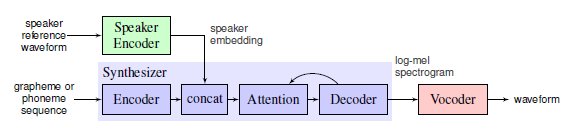
\includegraphics[width=\textwidth]{chapters/chapter2/sv2tts.png}
        \caption{Architecture of SV$_2$TTS adapted from \cite{jia_transfer_2019}}
        \label{fig:sv2tts}
    \end{figure}

    \textbf{Example with figure created by the author}:
    
    \begin{figure}[htbp]
        \centering
        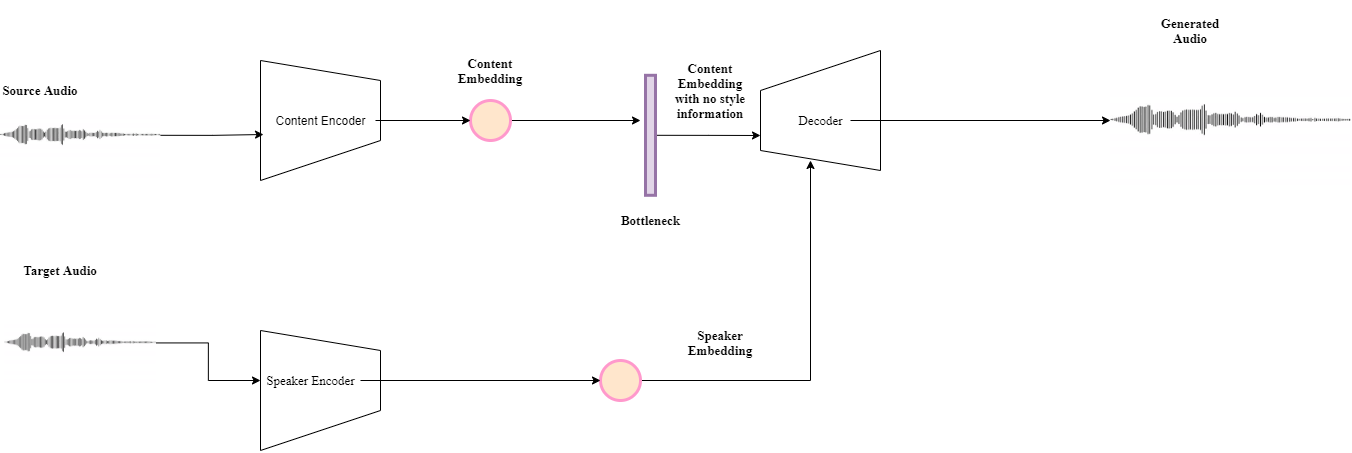
\includegraphics[width=\textwidth]{chapters/chapter2/autovc.png}
        \caption{Architecture of AutoVC}
        \label{fig:autovc}
    \end{figure}
    
   When working with figures, you may use either \verb|\linewidth| or \verb|\textwidth| to define the width of your figure, depending on your layout requirements. Additionally, you have the option to specify the dimensions of the figure by explicitly setting the \emph{width} or \emph{height} in centimeters or other units.
    
    
    When working with tables, the titles should be just \textbf{above} the table. Since tables cannot be divided between pages, they are usually best placed at the top of the page closest to their first reference. To achieve this correct “floating” positioning, use the \textbf{table} environment to wrap the table and its caption. The table's data should be placed within the \textbf{tabular} environment to ensure proper alignment in rows and columns, including any necessary horizontal and vertical lines.

    
    \begin{table}
        \centering
        \caption{A table \LaTeX\ with sample table commands}
        \begin{tabular}{c c c}
            \hline
            
            \textbf{Command} & \textbf{A Number} & \textbf{Comments}\\
            \hline 
            \hline
            
            \verb|\author| & 100 & Author\\
            \hline
            \verb|\table| & 300 & For tables\\
            \hline
            \verb|\table*| & 400 & For wider tables \\

            \hline
        \end{tabular}
        
        \label{tab:tab_mos}
    \end{table}

    Apart from the tabular environment you can use \textbf{tabulax} for more complex tables.

    \begin{table}
        \centering

        \caption{Sample complex table adapted from \cite{yamoah_deep_2022}. Use this to get a sense of how to create and format complex tables for your Capstone.}

        \begin{tabularx}{\textwidth}{>{\centering\arraybackslash}X|>{\centering\arraybackslash}X|>{\centering\arraybackslash}X|>{\centering\arraybackslash}X}
        \cline{2-4\emph{}}
        
        \multicolumn{4}{c}{\textbf{Participant Perception}} \\
        \cline{2-4\emph{}}
        \multicolumn{1}{c}{}& \multicolumn{1}{c}{\textbf{Fake}}&\multicolumn{1}{c}{\textbf{Real}}&\multicolumn{1}{c}{\textbf{Undecided}}\\
        \hline\hline
        
        \textbf{Experiment I} & 100\% & 0\% & 0\%\\
        \hline
        \textbf{Experiment II} & 90\% & 10\% & 0\%\\
        \hline
        \textbf{Experiment III} & 40\% & 20\% & 40\%\\
        \hline
        \textbf{Experiment IV} & 30\% & 70\% & 0\%\\
        \hline
        \textbf{Experiment V} & 70\% & 30\% & 0\%\\
        \hline
        \textbf{Experiment VI} & 90\% & 10\% & 0\%\\
        \hline
        \textbf{Experiment VII} & 40\% & 40\% & 20\%\\
        \hline
        \textbf{Experiment VIII} & 60\% & 40\% & 0\%\\
        \hline
        \textbf{Experiment IX} & 10\% & 20\% & 70\%\\
        \hline
        \textbf{Experiment X} & 20\% & 60\% & 20\%\\
        \hline
        \textbf{Experiment XI} & 30\% & 70\% & 0\%\\
        \hline
        \textbf{Experiment XII} & 20\% & 50\% & 30\%\\
        \hline
        
        \end{tabularx}
        
        \label{tab:tab_percep}
    \end{table}
    
    Finally, number figures and tables according to the chapter they are in.  For example, Figure 3.1: High-level system architecture or Table 4.1: Execution time of the algorithm for different problem sizes. However, if you are using this template it handles it for you but keep this in mind when editing in MS Word.
    
    \emph{Figure captions and Table titles should use “sentence case” (i.e. only the 1st word and proper nouns need to start with a capital letter) rather than “title case” (i.e. all words starting with a capital letter)}

    \item \emph{Code and algorithm listings:} For code and algorithm listings, use \verb|Courier 11pt| font. However, note that long code listings are typically not included in the main body of the report.

    \item  \emph{References:} Use the ACM referencing style. Ensure that both in-text citations and the reference list adhere to the specified style. The bibliography should be included in \verb|main.tex| using the appropriate commands, positioned just before \verb|\end{document}|. This ensures the proper formatting and placement of your references within the document. The commands ensuring this works as expected are:
        \begin{quote}
            \verb|\bibliographystyle{acm}|\\
            \verb|\begin{flushleft}|\\
                \verb|    \bibliography{references}|\\
            \verb|\end{flushleft}|
        \end{quote}

    To do an in-text citation use the command \verb|\cite{bibentry||. Examples: \cite{nguyen_deep_2021}, citing more than one bibentry in-text, \cite{ahamad_accentdb:_2020, yamoah_deep_2022, arik_deep_2017}. All bib entires are placed in the file \verb|references.bib|. If you do not know how to create bib entries you can use the website \href{https://zbib.org/}{\color{blue}{zoterobib}}.

    \item \emph{Appendices:} If your work requires an appendix, include it before the \verb|\end{document}| command in your source document. Begin the appendix by using the \verb|\appendix| command. Keep in mind that in accordance with ACM formatting, sections within the appendix are lettered rather than numbered.

    An example Appendix is included for your perusal.
    

        
\end{itemize}
